%%%%%%%%%%%%%%%%%%%%%%%%%%%%%%%%%%%%%%%%%%%%%%%%%%%%%%%%%%%%%%%%%%%%%%%%%%%%%%%%%%%%%
% PACOTES                                                                           %
%%%%%%%%%%%%%%%%%%%%%%%%%%%%%%%%%%%%%%%%%%%%%%%%%%%%%%%%%%%%%%%%%%%%%%%%%%%%%%%%%%%%%
\documentclass[a4paper,12pt]{article}

%-----------------------------------------------------------------------------------%
% LAYOUT DA PÁGINA                                                                  %
%-----------------------------------------------------------------------------------%
\usepackage[top=2.5cm, bottom=2.5cm, left=2.5cm, right=2.5cm]{geometry}
%\usepackage{fancyhdr} % Permite controlar como são exibidos os cabeçalhos

%-----------------------------------------------------------------------------------%
% FORMATAÇÃO DO TEXTO                                                               %
%-----------------------------------------------------------------------------------%
%\usepackage{setspace} % Permite definir o espaçamento entre linhas

%-----------------------------------------------------------------------------------%
% PACOTES DE IMAGENS                                                                %
%-----------------------------------------------------------------------------------%
\usepackage[pdftex]{graphicx}
\pdfsuppresswarningpagegroup=1 % A warning issued when several PDF images are
% imported in the same page. Mostly harmless, can be almost always supressed.
%\usepackage[pstarrows]{pict2e} % Amplia as funcionalidades do ambiente picture
\usepackage{tikz}
\usetikzlibrary{shapes, arrows, arrows.meta}

%-----------------------------------------------------------------------------------%
% PACOTES DE TABELAS                                                                %
%-----------------------------------------------------------------------------------%
\usepackage{array} % Facilita a formatação de tabelas
%\usepackage{multirow} % Permite criar células que ocupam várias linhas em uma tabela
\usepackage{longtable} % Permite criar tabelas que quebram de página

%-----------------------------------------------------------------------------------%
% PACOTES MATEMÁTICOS DE BASE                                                       %
%-----------------------------------------------------------------------------------%
\usepackage{amsfonts,amstext,amscd,bezier,amsthm,amssymb}
\usepackage[centertags]{amsmath}

%-----------------------------------------------------------------------------------%
% PACOTES DE SÍMBOLOS MATEMÁTICOS                                                   %
%-----------------------------------------------------------------------------------%
\usepackage{mathtools} % Símbolos matemáticos extras. (ex.: \xrightharpoon)
%\usepackage[integrals]{wasysym} % Muda o estilo das integrais, além de outros
%                                 símbolos extras
%\usepackage[nice]{nicefrac} % Permite o uso de frações "melhores". Usar \nicefrac{}{}

%-----------------------------------------------------------------------------------%
% PACOTES DE FONTES MATEMÁTICAS                                                     %
%-----------------------------------------------------------------------------------%
%\usepackage{mathbbol} % Quase todos os símbolos com \mathbb
%\usepackage{bbm} % Extensão dos símbolos de \mathbb. Usar comando \mathbbm
%\usepackage{calrsfs} % Muda o estilo de \mathcal
%\usepackage[mathcal]{euscript} % Muda o estilo de \mathcal

%-----------------------------------------------------------------------------------%
% PACOTES DE CODIFICAÇÃO DE FONTES                                                  %
%-----------------------------------------------------------------------------------%
\usepackage[utf8]{inputenc} % Permite o uso de caracteres ISO 8859-1, incluindo os
%                               caracteres acentuados diretamente.
\usepackage[T1]{fontenc} % Uso de fontes T1, necessário para tratar caracteres
%                          acentuados como um único bloco.

%-----------------------------------------------------------------------------------%
% PACOTES DE LÍNGUAS                                                                %
%-----------------------------------------------------------------------------------%
\usepackage[french]{babel} % Seleciona a língua do documento, definindo nomes de
%                              seções, nome do índice, da bibliografia, etc. Em caso
%                              de documento com mais de uma língua, a padrão é a
%                              última.
\NoAutoSpaceBeforeFDP % Utilizar em francês se quiser evitar espaços antes de :

%-----------------------------------------------------------------------------------%
% PACOTES DE BIBLIOGRAFIA                                                           %
%-----------------------------------------------------------------------------------%
%\usepackage{babelbib} % Permite definir a língua das entradas da bibliografia. Usar
%                       [fixlanguage] para uma mesma língua para todas as entradas e
%                       \selectbiblanguage{} para definir a língua. Um estilo compa-
%                       tível com babelbib deve ser usado (ex: babplain)
\usepackage{cite} % Organiza os elementos citados dentro de um mesmo \cite.

%-----------------------------------------------------------------------------------%
% PACOTES DE FONTES                                                                 %
%-----------------------------------------------------------------------------------%
% Computer Modern (fonte padrão)                                                    %
% - - - - - - - - - - - - - - - - - - - - - - - - - - - - - - - - - - - - - - - - - %
%\usepackage{ae} % A usar com a fonte padrão do LaTeX quando forem gerados PDFs, para
%                 corrigir erros de visualização

% Computer Modern Bright (sans serif)                                               %
% - - - - - - - - - - - - - - - - - - - - - - - - - - - - - - - - - - - - - - - - - %
%\usepackage{cmbright}

% Times New Roman                                                                   %
% - - - - - - - - - - - - - - - - - - - - - - - - - - - - - - - - - - - - - - - - - %
%\usepackage{mathptmx} % Muda texto e modo matemático
%\usepackage{times} % Apenas texto, não muda modo matemático

% Arial                                                                             %
% - - - - - - - - - - - - - - - - - - - - - - - - - - - - - - - - - - - - - - - - - %
%\usepackage[scaled]{uarial} % Arial como fonte sans serif padrão

% Palatino                                                                          %
% - - - - - - - - - - - - - - - - - - - - - - - - - - - - - - - - - - - - - - - - - %
%\usepackage{mathpazo} % Muda texto e modo matemático
%\usepackage{palatino} % Apenas texto, não muda modo matemático

% Concrete                                                                          %
% - - - - - - - - - - - - - - - - - - - - - - - - - - - - - - - - - - - - - - - - - %
%\usepackage{ccfonts} % Texto: Concrete; Matemático: Concrete Math
%\usepackage{ccfonts, eulervm} % Texto: Concrete; Matemático: Euler

% Iwona                                                                             %
% - - - - - - - - - - - - - - - - - - - - - - - - - - - - - - - - - - - - - - - - - %
%\usepackage[math]{iwona} % Texto e modo matemático: Iwona

% Kurier                                                                            %
% - - - - - - - - - - - - - - - - - - - - - - - - - - - - - - - - - - - - - - - - - %
%\usepackage[math]{kurier} % Texto e modo matemático: Kurier

% Antykwa Póltawskiego                                                              %
% - - - - - - - - - - - - - - - - - - - - - - - - - - - - - - - - - - - - - - - - - %
%\usepackage{antpolt} % Texto: Antykwa Póltawskiego; Matemático: nenhum
                     % Usar fontenc = QX ou OT4

% Utopia                                                                            %
% - - - - - - - - - - - - - - - - - - - - - - - - - - - - - - - - - - - - - - - - - %                     
%\usepackage{fourier} % Texto: Utopia; Matemático: Fourier

% KP Serif                                                                          %
% - - - - - - - - - - - - - - - - - - - - - - - - - - - - - - - - - - - - - - - - - %
\usepackage{kpfonts}

%-----------------------------------------------------------------------------------%
% CORES                                                                             %
%-----------------------------------------------------------------------------------%
\usepackage{color}
\definecolor{darkgreen}{rgb}{0,0.5,0}
\definecolor{darkmagenta}{rgb}{0.5,0,0.5}
\definecolor{darkgray}{rgb}{0.5,0.5,0.5}
\definecolor{darkblue}{rgb}{0.2,0.2,0.4}
\definecolor{darkred}{rgb}{0.6,0.15,0.15}
\definecolor{gray}{rgb}{0.65,0.65,0.65}
\definecolor{lightgray}{rgb}{0.8,0.8,0.8}
\definecolor{lightblue}{rgb}{0.5,0.5,1}
\definecolor{lightgreen}{rgb}{0.5,1,0.5}
\definecolor{deadred}{rgb}{0.7, 0.2, 0.2}
\definecolor{deadblue}{rgb}{0.2, 0.2, 0.7}

%-----------------------------------------------------------------------------------%
% PACOTES DIVERSOS                                                                  %
%-----------------------------------------------------------------------------------%
\usepackage{icomma} % Permite uso de vírgula como separador decimal
\usepackage{url} % Pacote para não ter problemas com URLs. Usar \url{}
%\usepackage{randtext} % Troca a ordem de letras de uma frase (útil com e-mails em
                      % PDFs a serem publicados on-line.
\usepackage[hidelinks]{hyperref}
%\usepackage{showkeys} % Para mostrar o nome dos labels
\usepackage{enumitem} % Facilita o uso de listas, inclusive referências a itens de
                      % listas.
%\usepackage[absolute]{textpos} % Posição absoluta de texto na página
%\usepackage{pdfpages} % Permite incluir documentos em PDF no arquivo
%\usepackage{refcheck} % Verifica as referências procurando por
%                      % labels não usados ou equações numeradas sem labels.
%                      % Verificar o arquivo .log e procurar por RefCheck.
\usepackage[french, onelanguage]{algorithm2e}

%%%%%%%%%%%%%%%%%%%%%%%%%%%%%%%%%%%%%%%%%%%%%%%%%%%%%%%%%%%%%%%%%%%%%%%%%%%%%%%%%%%%%
% CONFIGURAÇÕES                                                                     %
%%%%%%%%%%%%%%%%%%%%%%%%%%%%%%%%%%%%%%%%%%%%%%%%%%%%%%%%%%%%%%%%%%%%%%%%%%%%%%%%%%%%%

%-----------------------------------------------------------------------------------%
% FORMATAÇÃO DO TEXTO                                                               %
%-----------------------------------------------------------------------------------%
%\onehalfspacing % Espaçamento 1 1/2 (definido no pacote setspace)

%-----------------------------------------------------------------------------------%
% DEFINIÇÃO DE AMBIENTES MATEMÁTICOS                                                %
%-----------------------------------------------------------------------------------%
%\theoremstyle{plain}
%\newtheorem{theo}{Teorema}[section]
%\newtheorem{lemm}[theo]{Lema}
%\newtheorem{coro}[theo]{Corolário}
%\newtheorem{prop}[theo]{Proposição}
%\theoremstyle{definition}
%\newtheorem{defi}[theo]{Definição}
%\newtheorem{remq}[theo]{Observação}
%%\newtheorem{expl}[theo]{Exemplo}
%\newenvironment{expl}%
%  {\refstepcounter{theo}%
%    \begin{list}{}{%
%    \setlength{\topsep}{0pt}%
%    \setlength{\leftmargin}{\parindent}%
%    \setlength{\rightmargin}{0pt}%
%    \setlength{\listparindent}{\parindent}%
%    \setlength{\itemindent}{0pt}%
%    \setlength{\parsep}{\parskip}}%
%    \item[]{\bf Exemplo \thetheo. }}%
%  {\hspace*{\fill} $\square$ \end{list} \medskip}
%\newenvironment{solu}%
%  {\noindent {\bf Solução. }\small}%
%  {\hspace*{\fill} $\square$ \normalsize \medskip}
%\newenvironment{dems}[1][Demonstração]%
%  {\begin{list}{}{%
%    \setlength{\topsep}{0pt}%
%    \setlength{\leftmargin}{\parindent}%
%    \setlength{\rightmargin}{0pt}%
%    \setlength{\listparindent}{\parindent}%
%    \setlength{\itemindent}{0pt}%
%    \setlength{\parsep}{\parskip}}%
%    \item[]{\bf #1. }}%
%  {\hspace*{\fill} $\blacksquare$ \end{list} \medskip}


%-----------------------------------------------------------------------------------%
% DEFINIÇÃO DE COMANDOS MATEMÁTICOS                                                 %
%-----------------------------------------------------------------------------------%
%\newcommand*\diff{\mathop{}\!\mathrm{d}}

%\newcommand{\norm}[1]{\left\lVert #1\right\lVert} % Norma
%\newcommand{\abs}[1]{\left\lvert #1\right \rvert} % Valor absoluto
%\newcommand{\floor}[1]{\left\lfloor #1 \right\rfloor} % Arredondar para baixo
%\newcommand{\ceil}[1]{\left\lceil #1 \right\rceil} % Arredondar para cima
\DeclarePairedDelimiter{\ceil}{\lceil}{\rceil}
\DeclareMathOperator*{\argmax}{argmax}

%-----------------------------------------------------------------------------------%
% NUMERAÇÃO DE ELEMENTOS                                                            %
%-----------------------------------------------------------------------------------%
%\numberwithin{table}{section}
%\numberwithin{table}{subsection}
%\numberwithin{figure}{section}
%\numberwithin{figure}{subsection}
%\numberwithin{equation}{section}
%\numberwithin{equation}{subsection}
%\numberwithin{theo}{chapter}
%\numberwithin{theo}{subsection}

% Maximal percentage of the page occupied by floats
\renewcommand\floatpagefraction{.9}
\renewcommand\topfraction{.9}
\renewcommand\bottomfraction{.9}
\renewcommand\textfraction{.1}
% Maximal number of floats per page
\setcounter{totalnumber}{50}
\setcounter{topnumber}{50}
\setcounter{bottomnumber}{50}

\makeatletter\renewcommand\subsection{\@startsection{subsection}{2}{\z@}%
{-2ex\@plus -1ex \@minus -.2ex}%
{1.5ex \@plus .2ex}%
{\normalfont\large\bfseries}}\makeatother

%%%%%%%%%%%%%%%%%%%%%%%%%%%%%%%%%%%%%%%%%%%%%%%%%%%%%%%%%%%%%%%%%%%%%%%%%%%%%%%%%%%%%
% ESTRUTURA DO DOCUMENTO                                                            %
%%%%%%%%%%%%%%%%%%%%%%%%%%%%%%%%%%%%%%%%%%%%%%%%%%%%%%%%%%%%%%%%%%%%%%%%%%%%%%%%%%%%%
\begin{document}

\pagestyle{plain}

\title{3I005 \\ TME 2--4 : Projet Exploration / Exploitation}
\author{Ariana Carnielli \\ Yasmine Ikhelif}
\date{}

\maketitle

\sloppy

\tableofcontents

\section{Introduction}

Ce mini-projet s'intéresse à la problématique de l'exploitation \emph{vs} exploration, qui consiste à choisir, parmi une quantité de ressources limitées, combien de ces ressources vont être utilisées pour explorer le problème, afin d'avoir plus de chances de trouver la meilleure solution possible, et combien seront utilisées pour exploiter cette meilleure solution trouvée. Si beaucoup de ressources sont dépensées pour l'exploration, on aura plus de chances de trouver une solution proche de l'optimale, mais moins de ressources disponibles pour son exploitation. De l'autre côté, arrêter l'exploration trop tôt peut conduire au choix d'une action sous-optimale pendant la phase d'exploitation, ce qui conduit à un gain plus petit à long terme.

Dans ce mini-projet, on illustre la problématique de l'exploitation \emph{vs} exploration dans trois situations. La première, décrite dans la Section \ref{SecBM}, s'intéresse à l'exemple des bandits-manchots. Il s'agit de considérer une machine à sous à $N$ leviers, chacun ayant une probabilité de victoire différente inconnue du joueur. L'objectif est de maximiser le gain, ce qui nécessite un bon équilibre entre l'exploration des différents leviers afin d'avoir une bonne estimation de la probabilité de gain de chacun et l'exploitation du meilleur levier. L'algorithme principal permettant cet équilibre est l'algorithme UCB, dont les détails sont donnés dans la Section \ref{SecBM}.

La deuxième situation considérée, décrite dans la Section \ref{SecMorpion}, est celle du jeu du morpion, où trois stratégies de jeu sont implémentées. La première consiste dans une stratégie purement aléatoire, la deuxième est une stratégie de Monte Carlo, qui explore les actions possibles de façon aléatoire et choisit la meilleure et la dernière, une stratégie de Monte Carlo Tree Search, qui utilise l'algorithme UCB pour optimiser l'exploration des actions possibles.

Finalement, ces mêmes algorithmes, ayant été codés de façon généraliste, sont appliqués à un jeu légèrement plus complexe que morpion, le jeu puissance 4. Les détails de l'implémentation et les résultats obtenus sont donnés dans la Section \ref{SecPuissance4}.

\section{Bandits-manchots}
\label{SecBM}

\subsection{Description}

On considère une machine à sous avec $N$ leviers, numérotés par les entiers de $0$ à $N-1$. Chaque levier, lorsqu'il est actionné, peut donner une récompense de $0$ ou $1$ de façon aléatoire. On suppose que tous les leviers sont indépendants, que deux actionnements différents du même levier sont aussi indépendantes, et que la récompense du levier $i$ suit une loi de Bernoulli de paramètre $\mu^i$ constant en temps.

On dispose de $T$ coups pour jouer à la machine à sous. À chaque coup $t \in \{0, \dotsc, T-1\}$ , on choisit une \emph{action} $a_t \in \{0, \dotsc, N-1\}$, qui représente le levier choisi pour ce coup, et on accumule le gain obtenu avec ce levier, noté par $r_t$. Ainsi, $r_t$ est une variable aléatoire suivant une loi de Bernoulli de paramètre $\mu^{a_t}$. L'objectif est de maximiser le gain total $G_T$ obtenu au bout de $T$ coups, $G_T = \sum_{t=0}^{T-1} r_t$. Comme $G_T$ est une variable aléatoire, on maximise son espérance, qui vaut
\[
\mathbb E(G_T) = \mathbb E\left(\sum_{t=0}^{T-1} r_t\right) = \sum_{t=0}^{T-1} \mathbb E(r_t) = \sum_{t=0}^{T-1} \mu^{a_t}.
\]
Ainsi, si les $\mu^0, \dotsc, \mu^{N-1}$ étaient connus, la stratégie maximisant son espérance serait de choisir
\[a_t = \argmax_{i \in \{0, \dotsc, N-1\}} \mu^i\]
pour tout $t \in \{0, \dotsc, T-1\}$. Si on note $\mu^\ast$ la valeur maximale de $\{\mu_0, \dotsc, \mu_{N-1}\}$ et $G_T^\ast$ la variable aléatoire $G_T$ avec la stratégie $a_t$ définie ci-dessus, le maximum de l'espérance de $G_T$ vaut $\mathbb E(G_T^\ast) = \sum_{t=0}^{T-1} \mu^\ast = T \mu^\ast$.

Comme les $\mu^i$ ne sont pas connus, la stratégie ci-dessus ne peut pas être utilisée en pratique. Pour une autre stratégie, on s'intéresse au regret $L_T$ du joueur au bout de $T$ coups, défini comme la différence entre l'espérance du gain obtenu avec la stratégie optimale ci-dessus et son gain réel, $L_T = \mathbb E(G_T^\ast) - G_T = T \mu^\ast - \sum_{t=0}^{T-1} r_t$. Cette définition est légèrement différente de celle donnée dans l'énoncé du projet car on utilise l'espérance de $G_T^\ast$ au lieu d'un $G_T^\ast$ aléatoire. Ce choix, arbitraire, a été fait pour assurer que, lorsque deux résultats identiques sont obtenus par deux joueurs, leur regret sera aussi identique.

On est alors confronté à un problème du type exploitation \emph{vs} exploration, où l'exploration consiste à tester les leviers afin d'estimer leurs paramètres $\mu^i$ et l'exploitation consiste à jouer le levier avec le plus grand paramètre $\mu^i$ estimé.

\subsection{Implémentation du jeu}
\label{SecImplementation}

L'implémentation de la machine à sous a été faite en stockant les leviers d'une machine comme un tableau de taille $N$ contenant les paramètres $\mu^0, \dots, \mu^{N-1}$ des $N$ machines. La fonction \verb@cree_machine@ permet de créer un tel tableau avec des paramètres choisis de façon aléatoire uniforme dans $[0, 1]^N$. Un coup du jeu est simulé par la fonction \verb@jouer@, qui prend en argument une machine et l'action / levier choisi et rend le gain correspondant au coup joué. Une stratégie pour le jeu est une fonction quelconque prenant en argument un tableau \verb@mu@ donnant la proportion de gains de chaque levier et un deuxième tableau \verb@Na@ contenant la quantité de coups jouées dans chaque levier, et qui renvoie un coup à jouer à la prochaine étape. Les $T$ coups d'une partie sont simulés par la fonction \verb@run@, qui prend en argument la machine, la stratégie et $T$ et qui utilise les fonctions précédentes pour simuler les $T$ coups, renvoyant à la fin les dernières versions des tableaux \verb@mu@ et \verb@Na@ et un tableau de taille $T$ avec le gain cumulé à chaque $t \in \{0, \dotsc, T-1\}$. La fonction \verb@run@ utilise la fonction auxiliaire \verb@mise_a_jour@ qui met à jour les tableaux \verb@mu@ et \verb@Na@ en fonction du levier choisi et du résultat obtenu.

\subsection{Stratégies}
\label{SecStrategies}

Dans ce projet, quatre stratégies ont été implémentées.

\begin{itemize}[label=\textbullet, leftmargin=*]
\item \textbf{Algorithme aléatoire.} Dans cet algorithme, le levier à jouer au coup suivant est choisi de façon aléatoire uniforme parmi les $N$ leviers disponibles. Il s'agit d'un algorithme qui fait uniquement une exploration des $N$ leviers sans utiliser aucune information obtenue pour exploiter le meilleur levier observé.

\item \textbf{Algorithme glouton.} L'idée de cet algorithme est de décomposer le jeu en deux phases bien distinctes, l'une avec uniquement de l'exploration et l'autre avec uniquement de l'exploitation. Dans la première, les $N$ leviers sont joués chacun la même quantité de fois, passée en argument à la stratégie, afin d'estimer les paramètres $\mu^i$ de chaque levier par la proportion de gains obtenue expérimentalement sur ce levier stockée dans le tableau \verb@mu@. Remarquons que cette estimation est justifiée par la loi des grands nombres, qui garantit que la proportion des gains obtenue expérimentalement avec le levier $i$ converge vers le paramètre $\mu^i$. Dans la deuxième phase, l'algorithme glouton exploite les informations obtenues en jouant toujours au levier correspondant au maximum du tableau \verb@mu@.

\item \textbf{Algorithme $\varepsilon$-glouton.} L'inconvénient de l'algorithme glouton est que le tableau \verb@mu@ contient uniquement des estimations de $\mu^i$, et pas leurs vraies valeurs, qui sont inaccessibles. Ainsi, si ces estimations sont mauvaises, ce qui peut arriver de façon aléatoire, on risque de passer toute la phase d'exploration en jouant un levier qui n'est pas l'optimal. Pour y remédier, l'algorithme $\varepsilon$-glouton modifie l'algorithme glouton en introduisant un paramètre $\varepsilon$ petit. À chaque coup, on a une probabilité $\varepsilon$ de choisir un levier au hasard, de façon uniforme parmi les $N$ leviers, et, avec une probabilité $1 - \varepsilon$, on joue comme dans l'algorithme glouton. Cela garantit que, même après la fin de la première phase de l'algorithme glouton, on continue à avoir un peu d'exploration pour essayer d'améliorer les estimations de \verb@mu@ et ainsi éviter de rester bloqué sur une action sous-optimale.

\item \textbf{Algorithme UCB.} L'algorithme $\varepsilon$-glouton permet de garder un peu d'exploration pendant la phase d'exploitation, mais cette exploration est faite de façon purement aléatoire. L'algorithme UCB cherche à faire une exploration de façon plus intelligente avec les informations disponibles. L'idée de cet algorithme est de choisir la prochaine action $a_t$ par la formule
\[a_t = \argmax_{i \in \{0, \dotsc, N-1\}} \left(\hat\mu_t^i + \sqrt{\frac{2 \log(t)}{N_i(t)}}\right),\]
où $\hat\mu_t^i$ est l'estimation de $\mu^i$ disponible à l'instant $t$ et $N_i(t)$ est la quantité de fois que le levier $i$ a été actionné jusqu'à l'instant $t$. Le terme $\sqrt{\frac{2 \log(t)}{N_i(t)}}$ est celui responsable pour l'exploration ; sans ce terme, cette formule est exactement celle utilisée dans la phase d'exploitation de l'algorithme glouton. La division par $N_i(t)$ indique que, plus on a joué avec le levier $i$, plus notre estimation $\hat\mu_t^i$ est proche de $\mu^i$. Le terme en $\log(t)$ garantit qu'on ne néglige pas complètement un levier : même si son estimation de $\hat\mu_t^i$ est très petite, s'il a été très peu joué, le terme $\sqrt{\frac{2 \log(t)}{N_i(t)}}$ augmente au cours du temps et il sera éventuellement rejoué, afin d'améliorer encore l'estimation de $\hat\mu_t^i$. Comme la croissance de $\log(t)$ est assez lente, ces explorations de leviers avec une estimation petite n'arrivent pas très souvent pour ne pas trop nuire à l'exploration. Remarquons aussi que, comme il y a une division par $N_i(t)$, il est nécessaire de jouer chaque levier au moins une fois avant de pouvoir appliquer cet algorithme, ce qui impose une phase d'exploration pendant au moins les $N$ premiers coups.
\end{itemize}

Ces quatre stratégies ont été implémentées comme quatre fonctions, \verb@algo_alea@, \verb@algo_glouton@, \verb@algo_glouton_e@ et \verb@algo_UCB@, prenant toutes en argument les tableaux \verb@mu@ et \verb@Na@ comme décrit dans la Section \ref{SecImplementation}. L'algorithme glouton prend aussi en argument facultatif la quantité de fois que chaque levier est joué pendant la phase d'exploitation et l'algorithme $\varepsilon$-glouton prend en argument facultatif la valeur de $\varepsilon$.

\subsection{Résultats}

La Figure \ref{FigResultsTemps} montre le gain et le regret en fonction de $t$ pour les quatre algorithmes décrits dans la Section \ref{SecStrategies}. Pour cette simulation, on a choisi une machine à $N = 5$ leviers, le paramètre de la loi de Bernoulli de chaque levier ayant été choisi de façon aléatoire uniforme dans $[0, 1]$. On a fait une simulation avec 100 parties, chacune avec $T = 100$ coups. On a choisi une phase d'exploration de 10 coups par levier (donc 50 coups au total) pour l'algorithme glouton et $\varepsilon = 0.1$ pour l'algorithme $\varepsilon$-glouton. Les courbes représentent les gains et regret moyens obtenus.

\begin{figure}[ht]
\centering
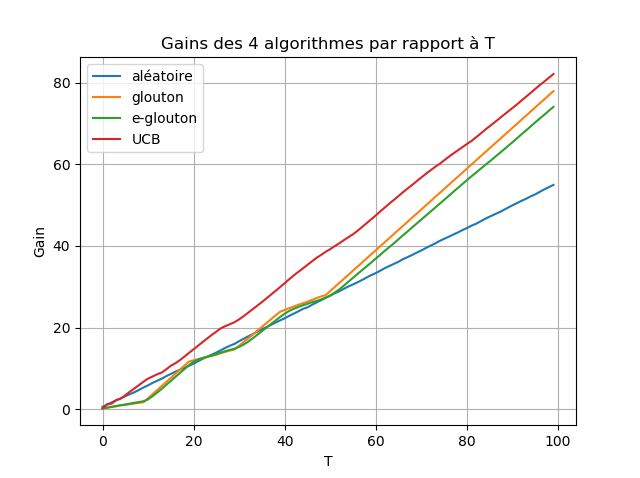
\includegraphics[width=0.75\textwidth]{Gain_T} \\
(a) \\
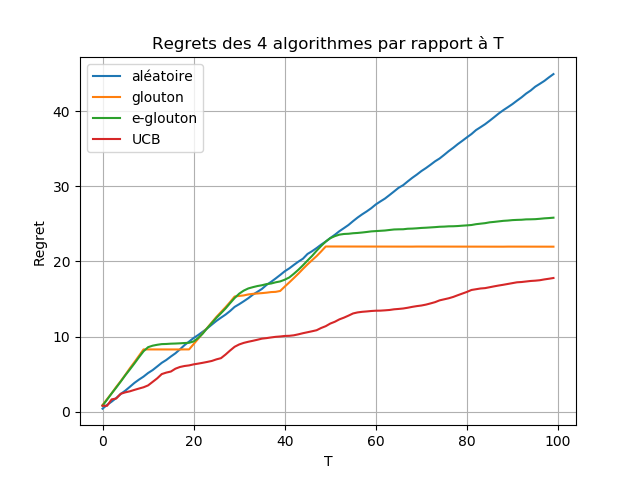
\includegraphics[width=0.75\textwidth]{Regret_T} \\
(b)
\caption{(a) Gain et (b) regret en fonction de $t$ pour chacun des quatre algorithmes de la Section \ref{SecStrategies}.}
\label{FigResultsTemps}
\end{figure}

On remarque que, dans cette simulation, l'algorithme UCB donne le gain maximal (et donc le regret minimal) parmi les quatre. On y voit aussi clairement que, jusqu'à $t = 50$, les algorithmes glouton et $\varepsilon$-glouton sont en phase d'exploration, la croissance de leur gain et de leur regret dépend ainsi de quel levier ils choisissent à chaque instant. À la fin de cette phase, l'algorithme glouton a trouvé le bon levier et donc son regret reste constant. Comme l'algorithme $\varepsilon$-glouton garde un peu d'exploration, son regret croit lentement après cette phase. L'algorithme UCB a un regret qui croit à chaque fois plus lentement, et de façon plus lente que les autres, lui donnant le plus petit regret à la fin.

\begin{figure}[ht]
\centering
\begin{tabular}{@{} >{\centering} m{0.5\textwidth} @{} >{\centering} m{0.5\textwidth} @{}}
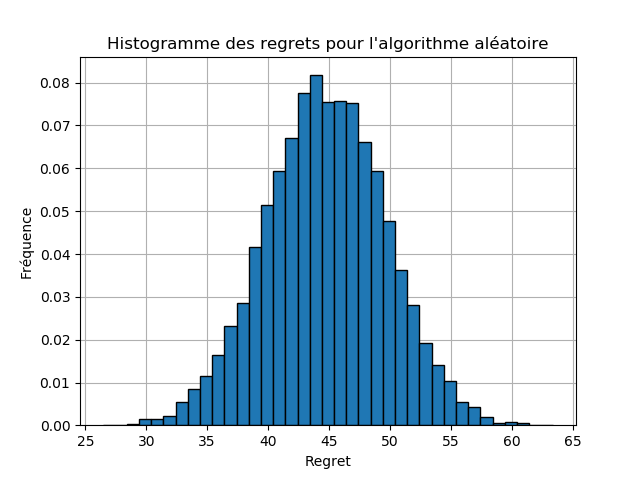
\includegraphics[width=0.5\textwidth]{Hist_alea} & 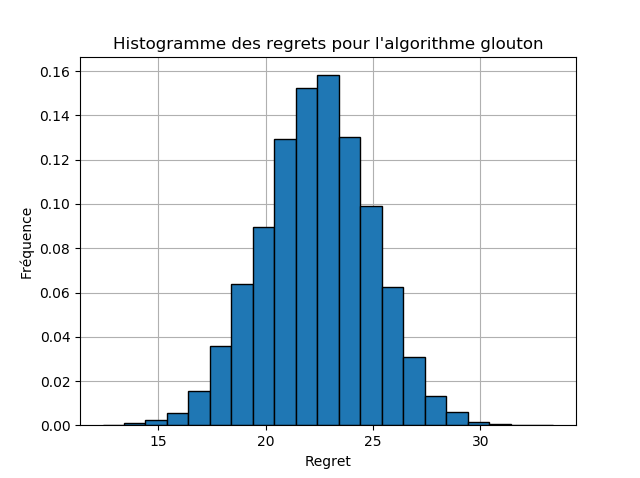
\includegraphics[width=0.5\textwidth]{Hist_glouton} \tabularnewline
(a) & (b) \tabularnewline
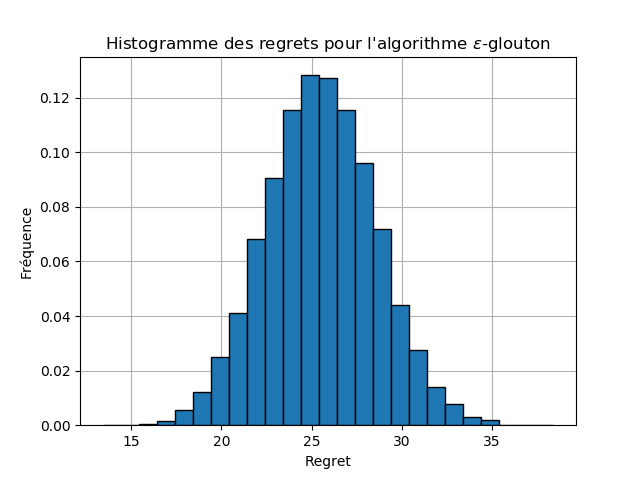
\includegraphics[width=0.5\textwidth]{Hist_glouton_e} & 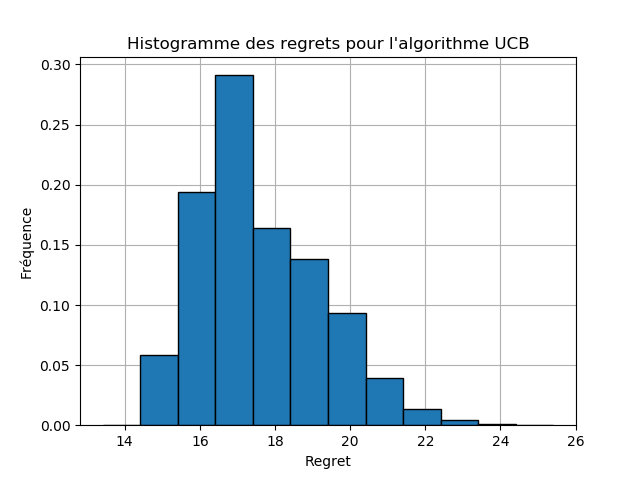
\includegraphics[width=0.5\textwidth]{Hist_UCB} \tabularnewline
(c) & (d) \tabularnewline
\end{tabular}
\caption{Histogramme des regrets au temps $T = 100$ après 10000 parties pour les algorithmes (a) aléatoire, (b) glouton, (c) $\varepsilon$-glouton et (d) UCB.}
\label{FigHist}
\end{figure}

La Figure \ref{FigHist} montre les histogrammes des regrets au temps $T = 100$ après 10000 parties pour chacun des 4 algorithmes, avec les mêmes paramètres que pour la Figure \ref{FigResultsTemps}. On y remarque que l'algorithme UCB donne toujours les plus petits regrets, qui sont concentrés entre 15 et 24. Les comportements des algorithmes glouton et $\varepsilon$-glouton sont similaires, mais avec un regret toujours plus grand pour le $\varepsilon$-glouton car, avec une phase d'exploration de 50 coups, l'algorithme glouton a beaucoup de chances de trouver le meilleur levier parmi les 5, et donc l'exploration faite par l'algorithme $\varepsilon$-glouton après les premiers 50 coups ne fait qu'augmenter son regret. Comme attendu, le regret de l'algorithme aléatoire est le pire des quatre.

On peut aussi comparer la précision des estimations des $\mu^i$ obtenues par les quatre algorithmes dans les simulations de la Figure \ref{FigResultsTemps}, données dans la Table \ref{TabMu}. On y remarque que l'algorithme aléatoire donne les meilleurs estimations, car cet algorithme ne fait que de l'exploration. L'algorithme UCB se concentre sur les leviers avec les plus grandes probabilités de gain, et ainsi ses estimations de $\mu^1$ et $\mu^4$ sont meilleures que les autres. L'algorithme glouton fait une estimation avec $10$ coups pour chaque levier et ensuite $50$ coups supplémentaires pour le meilleur levier estimé, ce qui lui donne une bonne estimation de $\mu^1$ mais une estimation plus mauvaise des autres $\mu^i$. L'algorithme $\varepsilon$-glouton améliore les estimations par rapport à l'algorithme glouton.

\begin{table}[ht]
\centering
\begin{tabular}{cccccc}
\hline\hline
 & $\mu^0$ & $\mu^1$ & $\mu^2$ & $\mu^3$ & $\mu^4$ \tabularnewline
\hline\hline
Valeurs réelles & $0.0225$ & $0.9499$ & $0.3808$ & $0.1185$ & $0.8149$ \tabularnewline
\hline
Algorithme aléatoire & $0.0205$ & $0.9502$ & $0.3688$ & $0.1236$ & $0.8139$ \tabularnewline
Algorithme glouton & $0.0270$ & $0.9420$ & $0.4070$ & $0.1340$ & $0.7833$\tabularnewline
Algorithme $\varepsilon$-glouton & $0.0212$ & $0.9396$ & $0.3772$ & $0.1136$ & $0.8131$\tabularnewline
Algorithme UCB & $0.0193$ & $0.9420$ & $0.3225$ & $0.0995$ & $0.7998$\tabularnewline
\hline\hline
\end{tabular}
\caption{Valeurs réelles des paramètres $\mu^i$ et valeurs estimées par chacun des algorithmes.}
\label{TabMu}
\end{table}

\section{Morpion}
\label{SecMorpion}

\subsection{Description et implémentation fournie}

Dans cette partie, on s'intéresse à des algorithmes pour jouer au morpion. Une implémentation de ce jeu a été fournie, basée sur quatre classes : une classe abstraite \verb@State@ permettant de représenter l'état générique d'un jeu de plateau à deux joueurs, une classe \verb@Jeu@ simulant un jeu générique, une classe \verb@MorpionState@ qui hérite de \verb@State@ et représente l'état d'un jeu de morpion, et une classe abstraite \verb@Agent@ permettant de représenter le comportement d'un agent. Un agent doit être capable, à partir de l'état courant du jeu, de renvoyer l'action qu'il choisit, c'est-à-dire la case qu'il marque avec son symbole, ce qui est fait par une méthode \verb@get_action@ prenant en argument l'état courant \verb@state@ et renvoyant l'action choisie.

\subsection{Stratégies}

Ce projet implémente trois stratégies différentes pour joueur au morpion : une stratégie aléatoire, une stratégie de Monte Carlo et une stratégie Monte Carlo Tree Search.

\begin{itemize}[label=\textbullet, leftmargin=*]
\item \textbf{Stratégie aléatoire.} La stratégie aléatoire, comme pour le problème des bandits-manchots de la Section \ref{SecBM}, n'utilise aucune information sur l'état du jeu outre les actions possibles et fait un choix aléatoire uniforme d'une de celles-ci. Si une stratégie aléatoire n'est pas intéressante par elle-même, elle sera utilisée comme une partie des deux autres stratégies.

\item \textbf{Stratégie Monte Carlo.} Les algorithmes de ce type consistent à remplacer une exploration exhaustive de l'espace de possibilités par un parcours d'un échantillonnage aléatoire uniforme de cet espace afin d'obtenir une approximation de quelle action est optimale sans tout calculer. Dans notre cas, à un état donné, pour chaque action possible, la stratégie de Monte Carlo simule plusieurs parties aléatoires (à l'aide de la stratégie aléatoire précédente) et calcule le taux de victoire de chaque action, choisissant celle avec le plus grand taux.

\item \textbf{Stratégie Monte Carlo Tree Search (MCTS).} La stratégie de Monte Carlo précédente consiste à regarder uniquement les actions possibles à partir de l'état courant et simuler des joueurs aléatoires ensuite. La stratégie Monte Carlo Tree Search s'intéresse plutôt à l'arbre de toutes les possibilités du jeu à partir de l'état courant et jusqu'à toutes les fins possibles du jeu. Cet algorithme cherche à parcourir cet arbre de façon intelligente, en choisissant en priorité les branches qui ont le plus de chances de conduire à une victoire. Plus précisément, il commence par explorer toutes les actions possibles à partir de l'état actuel au moins une fois et utilise l'algorithme UCB décrit dans la Section \ref{SecStrategies} pour choisir quelle branche explorer en priorité après, continuant ainsi jusqu'à un nombre prédéterminé d'explorations.
\end{itemize}

\subsection{Implémentations}

Dans cette partie, on présente de façon plus détaillée l'implémentation des stratégies Monte Carlo et Monte Carlo Tree Search. L'implémentation de l'algorithme aléatoire n'est pas décrite car elle est triviale.

\subsubsection{Monte Carlo}

L'algorithme de Monte Carlo a été implémenté en créant une classe \verb@AgentMC@ héritant de la classe \verb@Agent@. Elle implémente la méthode \verb@get_action@ en récupérant la liste d'actions possibles à partir de l'état courant et construisant deux dictionnaires indexés par les actions, l'un avec le nombre total de victoires pour chaque action et l'autre avec le nombre total de fois où cette action a été jouée. Pour garantir une exploration minimale, chaque action est jouée au moins une fois, avant de commencer une boucle où, à chaque tour, une action est choisie au hasard de façon uniforme, le prochain état du jeu est calculé, et ensuite cet état est joué par deux stratégies aléatoires afin de déterminer si cette action conduit à une victoire ou une défaite. À la fin une quantité prédéterminée de tours de boucle, la méthode renvoie l'action avec la plus grande proportion de victoires. La quantité de tours de boucle est fixée comme \verb@n@ fois le nombre d'actions possibles, où \verb@n@ est passé en argument facultatif à la classe.

\subsubsection{Monte Carlo Tree Search}

Comme la stratégie MCTS utilise un parcours d'arbre, on commence d'abord par implémenter une structure d'arbre adaptée à nos besoins. Cette structure se base sur la classe \verb@Noeud@, qui stocke l'état du jeu sur ce n\oe{}ud, son n\oe{}ud parent (ou \verb@None@ si c'est la racine), un dictionnaire avec ses n\oe{}uds fils, indexés par les actions qui conduisent à chaque fils, et les quantités de défaites et de parties jouées à partir de ce n\oe{}ud. Cela veut dire qu'un n\oe{}ud stocke la quantité de \emph{défaites} du joueur dont c'est le tour à ce n\oe{}ud.

La classe \verb@Noeud@, outre son constructeur, contient deux fonctions. La première, \verb@maj@, permet de mettre à jour le nombre de défaites de ce n\oe{}ud à partir d'un résultat d'une partie et propage cette information de façon récursive à son parent jusqu'à la racine. La deuxième, \verb@choix_ucb@, choisit le prochain n\oe{}ud à simuler à partir des principes de l'algorithme UCB. Si l'état est un état terminal, cette fonction renvoie le n\oe{}ud lui-même. Sinon, si son tableau avec ses enfants n'a pas encore été initialisé, cette fonction l'initialise. Elle parcourt ensuite le tableau d'enfants et, si elle trouve un enfant qui n'a pas encore été joué, la fonction lui retourne. Sinon, elle utilise l'algorithme UCB pour choisir un de ses enfants et fait un appel récursif à partir de cet enfant.

La classe principale de la stratégie MCTS est la classe \verb@AgentMCTS@, qui hérite de \verb@Agent@ et implémente la fonction \verb@get_action@. Elle initialise d'abord un n\oe{}ud \verb@racine@ lié à l'état courant, crée ses fils directs et joue une fois avec la stratégie aléatoire à partir de chacun d'eux. Ensuite, elle fait une boucle avec une quantité prédéterminée de tours. À chaque tour, la fonction \verb@choix_ucb@ est appelée sur la racine afin de déterminer un n\oe{}ud terminal ou qui n'a pas encore été joué. Un jeu est simulé à partir de ce n\oe{}ud et le résultat est propagé vers ses ascendants à l'aide de la fonction \verb@maj@. À la fin de cette boucle, la fonction regarde la quantité de défaites des fils de la racine et choisit celui avec le plus grand taux de défaites, ce qui correspond au plus grand taux de victoires pour le joueur de la racine. La quantité de tours de boucle est fixée comme \verb@n@ fois le nombre d'actions possibles, où \verb@n@ est passé en argument facultatif à la classe.

\subsection{Résultats}

Avant de présenter les résultats, rappelons que, dans le morpion, le premier joueur a un avantage naturel. Par exemple, lorsque le jeu se joue jusqu'à ce que la grille soit remplie, le premier joueur aura joué 5 coups, alors que le deuxième n'en aura joué que 4. En plus, le premier joueur a à sa disposition, au début, les 8 façons possibles de gagner (3 lignes, 3 colonnes et les deux diagonales), mais, après son premier coup, le deuxième joueur aura moins de façons possibles de gagner (4 si le premier joueur commence par le centre, 5 s'il commence par l'un des quatre coins ou 6 s'il commence dans l'une des quatre autres cases).

La Figure \ref{FigMorpion} montre l'évolution des proportions des victoires des joueurs 1 et 2 et de matchs nuls en fonction du nombre $N$ de parties jouées pour deux joueurs aléatoires. Elle illustre l'avantage donné par le jeu au premier joueur, qui a environ deux fois plus de chances de victoire que le deuxième joueur. Ces moyennes deviennent évidemment plus précises lorsque le nombre de parties jouées augmente.

\begin{figure}[ht]
\centering
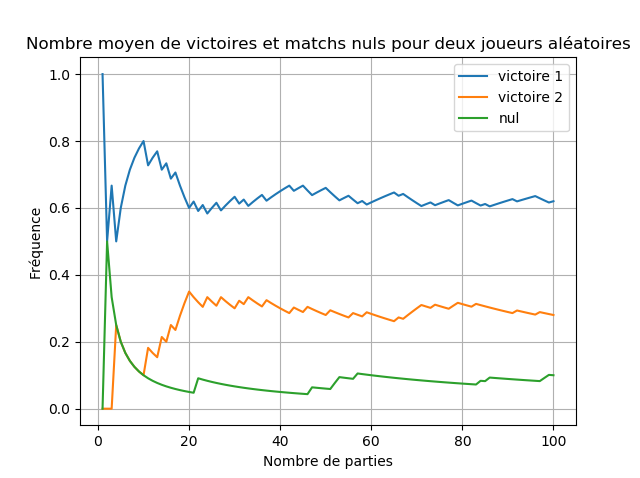
\includegraphics[width=0.7\textwidth]{TicTacToe}
\caption{Évolution des proportions de victoires des joueurs 1 et 2 et de matchs nuls entre deux joueurs aléatoires.}
\label{FigMorpion}
\end{figure}

La Table \ref{TabMorpion} présente les proportions de victoires des joueurs 1 et 2 et de matchs nuls au bout de $1000$ parties pour chaque combinaison possible des stratégies pour les deux joueurs. Pour les joueurs Monte Carlo et MCTS, le paramètre \verb@n@ déterminant la quantité de tours de boucle dans son implémentation a été fixée à $20$.

\begin{table}[ht]
\centering
\begin{tabular}{cc|ccc}
\hline\hline
Joueur 1 & Joueur 2 & Victoire joueur 1 & Match nul & Victoire joueur 2 \tabularnewline
\hline
Aléatoire & Aléatoire &     $57.2\%$ & $11.7\%$ & $31.1\%$ \tabularnewline
Aléatoire & Monte Carlo &   $14.5\%$ & $6.3\%$ & $79.2\%$ \tabularnewline
Aléatoire & MCTS &          $1.7\%$ & $10.3\%$ & $88.0\%$ \tabularnewline
Monte Carlo & Aléatoire &   $94.8\%$ & $3.8\%$ & $1.4\%$ \tabularnewline
Monte Carlo & Monte Carlo & $64.1\%$ & $15.7\%$ & $20.2\%$ \tabularnewline
Monte Carlo & MCTS &        $13.7\%$ & $45.8\%$ & $40.5\%$ \tabularnewline
MCTS & Aléatoire &          $99.3\%$ & $0.7\%$ & $0.0\%$ \tabularnewline
MCTS & Monte Carlo &        $83.9\%$ & $15.8\%$ & $0.3\%$ \tabularnewline
MCTS & MCTS &               $23.2\%$ & $76.2\%$ & $0.6\%$ \tabularnewline
\hline\hline
\end{tabular}
\caption{Proportions de victoires des joueurs 1 et 2 et de matchs nuls pour les différentes combinaisons possibles de stratégies dans le jeu du morpion.}
\label{TabMorpion}
\end{table}

La première ligne de la Table \ref{TabMorpion} met en évidence l'avantage du premier joueur et confirme les résultats montrés dans la Figure \ref{FigMorpion}. Elle montre aussi la hiérarchie entre les stratégies aléatoire, Monte Carlo et MCTS. Ainsi, même en tant que premier joueur, la stratégie aléatoire perd beaucoup contre Monte Carlo et presque à chaque fois contre MCTS, qui a un taux de $88\%$ de victoires malgré le désavantage d'être le second joueur. En premier joueur, la stratégie de Monte Carlo gagne presque à chaque fois contre l'aléatoire et a un bon taux de victoires contre elle-même, mais, contre MCTS, le plus probable est d'avoir un match nul, avec aussi une grande probabilité pour que MCTS gagne, même en second joueur. Lorsque MCTS est le premier joueur, il gagne presque systématiquement contre l'aléatoire, avec un taux très faible de matchs nuls et aucune défaite. Son taux de victoires contre Monte Carlo est lui aussi très élevé. Quand deux joueurs MCTS jouent l'un contre l'autre, la probabilité de match nul est assez élevée, et, lorsqu'il n'y a pas match nul, c'est presque toujours le premier joueur qui l'emporte. Cela se rapproche de la stratégie optimale pourle morpion, dans laquelle on a un match nul à coup sûr. Il est possible de se rapprocher de cette situation en augmentant le paramètre \verb@n@ de MCTS déterminant le nombre de tours de boucle, mais cela rend aussi ce joueur plus lent. Avec \verb@n = 20@, l'ensemble des simulations de la Table \ref{TabMorpion} a pris environ 30min pour s'exécuter, dont environ 20min pour le remplissage de ses trois dernières lignes.

Une amélioration envisageable du code serait de réutiliser l'arbre d'un coup à l'autre. En effet, à chaque fois que l'on demande son action à un joueur MCTS, il construit à partir de zéro l'arbre du jeu à partir de l'état actuel. Une fois son coup choisi et retourné, cet arbre n'est plus réutilisé, et un nouvel arbre est construit à partir de zéro à la prochaine fois qu'on lui demande une action. Pour garder de l'information entre un coup et l'autre, on pourrait stocker l'arbre comme variable d'instance pour le joueur et le mettre à jour à chaque coup joué. Pour cela, il faut prendre en compte le coup qu'il a joué et aussi le coup joué par l'autre joueur.

\section{Puissance 4}
\label{SecPuissance4}

\subsection{Description et implémentation}

Les algorithmes pour jouer au morpion de la Section \ref{SecMorpion} ont été appliqués au jeu Puissance 4. Ce jeu se joue sur une grille à 6 lignes et 7 colonnes et l'objectif d'un joueur est d'aligner 4 de ses pièces à l'horizontale, verticale ou diagonale. Les joueurs ne peuvent pas placer leurs pièces de façon arbitraire : à son tour, un joueur choisit une colonne et y place sa pièce obligatoirement dans la ligne la plus en bas possible.

Les stratégies implémentées pour le morpion marchent sans aucune modification pour le jeu Puissance 4, car elles se basent sur les méthodes de la classe abstraite \verb@State@. Ainsi, pour implémenter ce jeu, il suffit d'implémenter une classe héritant de \verb@State@, que l'on a appelée \verb@Puissance4State@. Dans cette classe, il suffit d'implémenter les fonctions \verb@get_actions@, qui donnent les actions possibles d'un joueur à son tour, \verb@win@, qui détermine si l'un des deux joueurs a gagné le jeu et, si oui, lequel, et \verb@stop@, qui détermine si le jeu est terminé, soit par la victoire d'un des deux joueurs ou par le remplissage complet de la grille.

\subsection{Résultats}

Comme pour le jeu de morpion, le jeu Puissance 4 donne un avantage au premier joueur, ce qui a été découvert en 1988 de façon indépendante et presque simultanée par James Dow Allen et Victor Allis, mais cet avantage est moins significative que pour le jeu de morpion. Nous avons simulé $500$ parties pour chaque combinaison possible de stratégies pour les deux joueurs d'un jeu de Puissance 4, les proportions de victoires des joueurs 1 et 2 et de matchs nuls étant représentés dans la Table \ref{TabP4}.

\begin{table}[ht]
\centering
\begin{tabular}{cc|ccc}
\hline\hline
Joueur 1 & Joueur 2 & Victoire joueur 1 & Match nul & Victoire joueur 2 \tabularnewline
\hline
Aléatoire & Aléatoire &     $49.4\%$ & $5.0\%$ & $45.6\%$ \tabularnewline
Aléatoire & Monte Carlo &   $5.6\%$ & $0.4\%$ & $94.0\%$ \tabularnewline
Aléatoire & MCTS &          $0.0\%$ & $0.2\%$ & $99.8\%$ \tabularnewline
Monte Carlo & Aléatoire &   $95.8\%$ & $0.2\%$ & $4.0\%$ \tabularnewline
Monte Carlo & Monte Carlo & $49.0\%$ & $4.6\%$ & $46.4\%$ \tabularnewline
Monte Carlo & MCTS &        $7.2\%$ & $4.6\%$ & $88.2\%$ \tabularnewline
MCTS & Aléatoire &          $100.0\%$ & $0.0\%$ & $0.0\%$ \tabularnewline
MCTS & Monte Carlo &        $94.0\%$ & $3.6\%$ & $2.4\%$ \tabularnewline
MCTS & MCTS &               $43.8\%$ & $17.4\%$ & $38.8\%$ \tabularnewline
\hline\hline
\end{tabular}
\caption{Proportions de victoires des joueurs 1 et 2 et de matchs nuls pour les différentes combinaisons possibles de stratégies dans le jeu Puissance 4.}
\label{TabP4}
\end{table}

On remarque, dans le match entre deux joueurs aléatoires, l'avantage du premier joueur, qui est cependant beaucoup moins importante que dans le cas du morpion. Contre les stratégies Monte Carlo ou MCTS, le joueur aléatoire perd presque à chaque fois, peu importe s'il est le premier ou deuxième joueur. Lorsque les deux joueurs suivent la stratégie Monte Carlo, les résultats ne sont pas très différents que dans le cas de deux joueurs aléatoires. Encore une fois, le joueur MCTS est celui avec la meilleure stratégie, gagnant presque toutes les parties contre les autres joueurs. Le cas entre deux joueurs MCTS est aussi celui avec le plus d'occurrences de matchs nuls.


\section{Conclusion}

Ce rapport a permis, dans la Section \ref{SecBM}, de mettre en évidence la problématique de l'exploitation \emph{vs} exploration à travers l'exemple des bandits-manchots, qui illustre bien l'intérêt d'un algorithme équilibrant exploration et exploitation comme l'algorithme UCB. On a également pu remarquer, dans les Sections \ref{SecMorpion} et \ref{SecPuissance4}, que l'utilisation de cet algorithme dans la stratégie Monte Carlo Tree Search permet d'obtenir des joueurs très performants.

\end{document}
